\documentclass{scrartcl}
\usepackage{dominatrix}
\usepackage{tikz}
\usepackage{pgfplots}
\pgfplotsset{
	every axis/.append style={font=\small},
	compat=newest
}
\begin{document}
   
    CS 5220 Introduction to Parallel Programming \hfill Fall 2015 \\
    Kenneth Lim (\href{mailto:kl545@cornell.edu}{kl545}), Scott Wu (\href{mailto:ssw74@cornell.edu}{ssw74}), Robert Chiodi (\href{mailto:rmc298@cornell.edu}{rmc298}), Ravi Patel (\href{mailto:rgp62@cornell.edu}{rgp62})  \hfill Final Project \hspace{-3ex}



    \section{Introduction}

    \subsection{Smooth Particle Hydrodynamics (SPH)}

    \subsubsection{Purpose}
    The purpose of this project is to implement a Smoothed Particle Hydrodynamics based on \href{http://mmacklin.com/pbf\_sig\_preprint.pdf}{Position Based Fluids} (Macklin, Muller 2013). Since the goal of the paper is geared towards real time use, some portions of the algorithm will sacrifice accuracy for speed. Finally, we will be analyzing and parallelizing the algorithm to further improve performance.
        
    \subsection{Code Bases}
    
    \subsubsection{Fortran Code}
    The Fortran code is based off of an SPH code used by Professor Bindel in the spring of 2014 for CS 5220: Applications of Parallel Computers. This code was selected because it directly referenced the solution of the relevant equation (Navier-Stokes) and discussed treatments required to have a working code. SPH can be very unstable without sufficient parameter tuning and having the reference code available allowed easier creation of a serial program that could then be parallelized. Several modifications and additions have been made to this code, as well as it being transferred to Fortran, that will be discussed later. The main contributions taken from the reference code were the leap-frog time integration scheme, handling of walls via damping coefficients, and the recalculation of mass during initialization to have particle densities near the particle reference density. The additions and transfer to Fortran for the serial code led to an order of magnitude speed up for the dam break problem created in the C version using the ``box indicator''. 
    
    The initialization of the Fortran code is handled via an initial text file generated with a python script. This text file contains the number of particles, the time step, the size of the particles, domain side length (with the domain being assumed cubic), frequency of visualization file output, final desired simulation time, and initial position and velocity of all particles. This is a very flexible format for initialization that allows easy rerunning of simulation conditions and the creation of a diverse problem set.
    
    
    \subsubsection{C Code}
    
    The C code is based off of the Java code from Professor James' assignment for CS 5643. This assignment was oriented towards speed and real-time simulation. The original skeleton code contained a GUI and simple particle system framework. For simplicity in the C implementation, all data structures and functions were kept as native data types in the global namespace. Like the Fortran code, the implementation reads from the same initialization files although with slightly different parameters. In the main program loop, the step size is further split into multiple substeps, although output was only written at the end of the whole step. The C implementation borrows ideas from the Fortran code such as collision damping and reference particle density to improve the stability of the simulation.
    
    \subsubsection{Algorithm Overview}
        
        In the simulation, our inputs are the initial positions and velocities of particles in a box. Then we take equal time steps, producing the same list of position and velocity outputs at each step.
        
        \begin{itemize}
        	\item At the beginning of each step, we compute candidate velocities and positions by taking an Eulerian step
        	\item We compute the neighbor's particles within a certain radius by placing them on a grid
        	\item Candidate velocities and positions are iteratively corrected
        	\begin{itemize}
        		\item Per iteration, we attempt to solve the incompressibility constraint
        		\item Meanwhile maintain the boundary conditions of the box, and apply velocity dampening if necessary
        		\item Update the candidate positions with those constraints
        	\end{itemize}
        	\item Using the new candidate positions, we update the candidate velocities
        	\item We apply vorticity confinement to maintain energy in the system
        	\item We apply viscosity to blur the velocities into a more coherent motion
        	\item Finally we update the positions and velocities with the candidate positions and velocities
        \end{itemize}
    
        
        
        \subsubsection{Performance Model}
        Each of the sections listed above must be executed sequentially. However, what can be parallelized are each of the individual steps.
        If we have $n$ particles, then the upper bound for our serial time per time step is:
        \\
        $$t_{forces} * n + t_{candidates} * n + t_{neighbors} * n^2 + t_{iterations} * n^2 +$$
        $$t_{vorticity} * n^2 + t_{viscosity} * n^2 + t_{update} * n$$
        \\
        This is a very pessimistic bound because the $n^2$ coefficient on most of the terms assume that all particles are neighbors of all other particles, which is never the case. If we let $a$ be the average number of neighbors per particle (which the simulation will eventually stabilize to), then our new model for serial time is:
        \\
        $$t_{f} * n + t_{c} * n + t_{nb} * n^2 + t_{iter} * n * a + t_{vo} * n * a + t_{vi} * n * a + t_{u} * n$$
        \\
        If we have $p$ processors, then our parallel time per time step is:
        \\
        $$(t_{f} * n + t_{c} * n + t_{nb} * n^2 + t_{iter} * n^2 + t_{vo} * n * a + t_{vi} * n * a + t_{u} * n) / p + t_{overhead}$$
        \\
        Although there are no major branches in the algorithm, there will still be synchronization overheads and small critical serial sections in a parallel implementation.
    
    \subsection{Writing of Visualization Files}
    The writing of visualization files is handled the same way in each code. At a specified frequency, by a certain number of time steps in the C version or an amount of simulated time in the Fortran version, a text file is written that contains the number of particles along with their position and velocity. The text files are numbered sequentially with integer tags in order to keep the proper time sequence. A python script we wrote, based loosely off of the visualizer script written for the wave-equation assignment, then plots each particle as a point on a 3D scatter plot and encodes the images together with \texttt{ffmpeg}.

    \section{Profiling and Serial Optimization}
  
  \subsection{Fortran Code}
  \subsubsection{Profiling}
  In order to profile the Fortran code, manual timing was implemented using the OpenMP function, \texttt{omp\_get\_wtime}. This was deemed sufficient due to the highly modular nature of the Fortran code, where the majority of subroutines called feature a nested do-loop that computes the effect of particle neighbors on each particle. For this profiling, the known fact about particle simulations was confirmed; neighbor finding is the predominant cost. In the naive version of the code, the neighbor finding routine takes several orders of magnitude longer per iteration. After optimizations, the neighbor finding routine was reduced to only being 10 times more expensive than any other routine per step, meaning in all cases it still remained the dominant bottle neck. For this reason, the neighbor finding routine was focused on in both the optimization and parallelization of the Fortran code. 
  
  \subsubsection{Optimizations}
  The optimizations of the serial program were primarily made through reorganization of the neighbor finding routine and encouraging vectorization by the compiler. Since the neighbor finding routine received the most attention and had the greatest impact on program speed,  this will be focused on first and will be addressed with the most detail.
  
  Naive neighbor finding is an $n^2$ operation that is known to be the predominant cost of SPH fluid simulations. In order to improve upon this, we used spatial binning to reduce the number of particles each particle checks to determine neighbors. The general algorithm can be written in pseudo-code as:
      \begin{itemize}
      	\item For each particle, its bin in the x, y, and z direction is calculated. During this, number of particles in each bin as well as the index of the particle in each bin is tracked.
      	\item Each bin is then iterated through, consisting of
	      	\begin{itemize}
	      		\item A particle in the bin is chosen
	      		\item The neighboring 26 bins are iterated through, as well as the particle's bin itself
	      		\item The distance between particles is calculated
	      		\item If the distance is less than the kernel size, the particle is a neighbor and added to a list of neighbors for that particle. The number of neighbors is also tracked.
	      	\end{itemize}
      \end{itemize}
   This handling of neighbors is much faster than the naive treating of neighbor finding, however it is still very costly. In order to reduce the cost further, the finding of neighbors can be handled in pairs, since it is known that if particle $j$ is a neighbor of particle $i$, then $i$ is a neighbor of $j$. This provides a significant speed up, however becomes complicated in parallel without an excessive amount of synchronization. Inherently this algorithm is hard to optimize for the compiler since it must be checked that the distance between particles is less than the kernel size. Additionally, if all bins are looped through together, if statements are required to ensure that ``bins'' outside of the simulation domain are not checked since this will lead to array bound issues. To address this issue, the iteration through bins was split up to first check bins along the domain boundaries, allowing the internal domain, which contains the majority of the bins, to be iterated through without checking bounds on neighboring spatial bins. Along with these algorithmic considerations, other simple computational considerations were incorporated, such as looping through bins using the smallest memory stride in the accessed arrays to take advantage of spatial cache locality.
   
	SPH fluid programs have an inherent particle symmetry implied which was used to reduce the amount of computational work needed to be performed. For the calculation of forces and density, the calculated force or density can be applied to the neighbor as well, halving the amount of naive work that would be performed when calculating distances and kernel coefficients. This work can be quite costly with complex expressions used for many of the kernels, allowing a significant saving of time relative to the time spent in those routines. Computing force and density contributions from neighbors in pairs also utilizes the working set better, using the neighbor information that is already loaded into cache. 
	
	In all areas of the code, efficient coding was strived for, pre-computing all constants that are used multiple times and allocating each array only once. One issue with this is the need to estimate the maximum number of neighbors a single particle will have in order to allocate the associated arrays once. This estimation has a significant impact the neighbor finding routine since it greatly effects the offset between non-data-sequential bins and can quickly lead to cache thrashing. For our final, optimized version of the code, we decided to estimate the maximum possible number of neighbors as 100 times a homogeneous distribution of particles, or
	\begin{equation}
	\mathrm{max\_part\_guess} = \frac{100 \; n}{\mathrm{nbinx} \times \mathrm{nbiny} \times \mathrm{nbinz}}
	\end{equation}
	This seemed to lead to quick and robust simulations. In the future, if we had more time, we would most likely implement a linked-list method in order to avoid having to preallocate arrays for neighbors.
	
	Memory alignment was also forced to 64-byte boundaries in order to aide the compiler in vectorization, something that Fortran is typically strong in. The compiler's vectorization report was used to ensure vectorization when possible, which once again provided some performance gain due to on-core parallelism.
	
	These optimizations discussed here sped the program up by a factor of 13 for a dam break with 2197 particles ran for 10,000 iterations; from 219 seconds to 16.9 seconds. The original program that managed to simulate the dam break in 219 seconds already incorporated the general algorithm discussed for spatial binning neighbor finding, however did not have optimized looping orders or allocations, showing the importance of proper memory management and cache use.
      
  \subsubsection{Compiler Flags}
  In order to have cross-platform portability of the program and ease of testing on Totient as well as locally, it was decided to use GNU's gfortran. Since accuracy in SPH for graphics is not of paramount performance, full optimization (\texttt{O3}) and \texttt{ffast-math} were used to allow quicker handling of floating point operations. Loop unrolling was also specifically requested with the \texttt{funroll-loops} compiler flag. As previously seen in past homework assignments, compiler flags provide a significant code speedup with minimal effort.
 
  \subsection{C Code}
  \subsubsection{Profiling}
          
          Serial profiling was done on a dam break simulation with 16000 particles.
          \[\begin{array}{lc}
          \mathrm{Forces:}     & 0.025267 s \\
          \mathrm{Candidates:} & 0.046138 s \\
          \mathrm{Neighbors:}  & 9.710008 s \\
          \mathrm{Iterations:} & 43.94977 s \\
          \mathrm{Vorticity:}  & 4.347007 s \\
          \mathrm{Viscosity:}  & 1.153325 s \\
          \mathrm{Update:}     & 0.046102 s \\
          \end{array}\]
          
          From here we observe that the majority of time is spent in solver iterations. Since we perform 10 iterations per step, this equates to around 4.4 seconds per iteration. Another large chunk of time is spent finding neighbors. Although binning particles takes O($n$) time, searching through the 27 surrounding bins is potentially an O($n^2$) operation if the majority of particles are clustered around an area.
          \newpage
              \subsubsection{Optimizations}

With the given compiler flags, we begin by optimizing the data structures in our code. In the initialization phase, we dynamically allocate arrays to the next largest multiple of 64 along with the aligned attribute. We also pass restrict keywords to functions so that the loops within them may be vectorized by the compiler.

Moving on to parallel optimizations, we focus on using OpenMP. Since only a few data accesses are overlapping (in particular ones relating to using neighbors), we can let all arrays be shared by default. In computing forces, each particle's force is cleared, and then the previous time step's vorticity force and gravitational force is applied. This is a simple parallel for loop, since no particle's forces overlap one another. Computing candidates is very similar in that each particle's candidate position and velocity is independent of other particles, requiring another parallel for.

Finding neighbors starts to cause issues when placing particles into bins. Bin access may be random, so we would like to lock a bin when accessed, but also not prevent other threads from locking on different bins. A critical or atomic pragma would not work, since it would cause all threads to lock. Instead we initialize an array of OpenMP mutexes equal to the number of bins, which is decided at initialization. Upon writing to a bin, we lock and unlock that bin's mutex. This way other threads can continue execution on other bins, while maintaining atomic updates on any single bin. From there, actually finding and assigning neighbors becomes a parallel for loop over the particles since the bins are only read.

Iterations must be computed one after another. Inside them, we can parallelize the solver, pressure and collision calculations. Since pressure depends on the lambda coefficient calculated in the solver, they must be done in different loops. However pressure and collisions are independent, and can be done within the same loop.

Vorticity takes two steps, one to compute the angular velocities, another to compute the correction forces. As mentioned previously, these forces are applied on the next time step. Angular velocity depends on the candidate linear velocities of neighbors. The correction force depends on angular velocity. Both loops may be parallelized over the particles. Viscosity must be performed after vorticity confinement because it modifies the candidate velocities. The final update uses candidate positions and velocities to update the final positions and velocities. Although these last few loops could be combined, we leave them in that order for timing and debugging purposes.

For timing OpenMP code, we used shared timing variables combined with \texttt{\#pragma omp single nowait}. The \texttt{nowait} clause prevents any synchronization barrier when calling \texttt{omp\_get\_wtime()}, since it is not necessary in this case.
          
          \subsubsection{Compiler Flags}
          We use the typical compiler flags with the Intel compiler, including O3, fast, ipo, AVX512 and restrict. These flags are taken from past assignments.
       

  
  \section{Parallelization}
  Both the C code and Fortran code were parallelized using OpenMP. Additionally, the Fortran code was parallelized using MPI in order to assess the capabilities of the two methods. In all cases, strong and weak scaling studies were performed to better understand the code's parallel efficiency. Here, we define strong scaling, strong scaling efficiency, and weak scaling by Equations~(3.1),~(3.2), and~(3.3), respectively,
  
  \begin{equation}
  \mathrm{Strong\;Scaling} = \frac{t_{\mathrm{serial}}}{t_{\mathrm{parallel}}}
  \label{eq:ss}
  \end{equation}
  
   \begin{equation}
  \mathrm{Strong\;Scaling\;Efficiency} = \frac{t_{\mathrm{serial}}}{t_{\mathrm{parallel}}} \frac{1}{p}    
   \label{eq:sse}
   \end{equation}
    
    \begin{equation}
      \mathrm{Strong\;Scaling} = \frac{t_{\mathrm{serial}}(n(p))}{t_{\mathrm{parallel}}(n(p),p)}  
    \label{eq:ws}
    \end{equation}
	 where $t_{\mathrm{serial}}$ is the time to solve the problem serially, $t_{\mathrm{parallel}}$ is the required time to solve the problem in parallel, and $p$ is the number of processors. It is important to note that for strong scaling, the problem size remains constant, however for weak scaling the problem size scales linearly with the number of processors.
  
  \subsection{Fortran Code}    
  The optimized Fortran code was parallelized separately in OpenMP and MPI in order to judge the effectiveness of both parallelization paradigms. For the size of our problems of interest, OpenMP appears to be superior due to its shared memory architecture reducing the number and cost of synchronizations significantly.
  \subsubsection{OpenMP}
  The parallelization of the Fortran code with OpenMP was primarily handled through the use of !\$OMP DO loops, !\$OMP WORKSHARE, and \$!OMP MASTER loops. The !\$OMP DO loops is the Fortran equivalent of C's \#pragma parallel for, and was the workhorse of our parallel implementation. The !\$OMP WORKSHARE command is analogous to !\$OMP DO, however is used to the implicit vectorization operations available in Fortran, such as vectorized copying of arrays. Lastly, \$!OMP MASTER was used to force serial execution of a section by the master thread, which was primarily used for the writing of visualization files.
  
  The parallelization of the neighbor finding routine required significant reorganization. The method presented previously in the serial optimization becomes too costly due to the synchronization required to ensure neighboring particles do not get counted twice when finding neighbors in pairs. To avoid this, neighbor finding was reverted to a less efficient, but synchronization-less method where neighbors are not accounted for in pairs.  Additionally, looping through bins in each direction is too small of a range to effectively parallelize. To fix this, the previously 3-nested bin iteration loop (x, y, z) was changed to a single loop of size nbinx $\times$ nbiny $\times$ nbinz where the bin in each direction is found through moduli. This loop then has chunks assigned via OpenMP dynamically, in order to help with the load balancing in the case of many successive empty bins. With neighbors found, the remainder of the code was parallelized using the !\$OMP DO and !\$OMP WORKSHARE commands.
  
  In order to assess the effectiveness of the parallelization, strong and weak scaling studies were performed. For clarification, in each study, the one processor case is the serial code without the serial optimizations, not the parallel code ran with one processor.
  
  \textbf{Strong Scaling:}
  The strong scaling study was performed for six test points, shown in Table~\ref{tab:fompss}, where we ensured to have one test case on more than 12 threads to assess the capability when threads were separated by physical chips. The strong scaling results itself can be seen in Figure~\ref{fig:ss_fort_omp}. Surprisingly decent strong scaling of over 50\% can seen for 2 threads, however this quickly drops off as more threads are added. We believe this scaling behavior is due to an increase in cache thrashing with the addition of more threads. Specifically in the neighbor finding routine, the checking of a neighbor requires the loading of position and spatial bin data, which will more quickly be removed from cache with other processors looking for neighbors who have data associated far away in the array. It may be possible to improve this performance through more intelligent work division and binning.
  
      \begin{table}
      	\begin{center}
      		\begin{tabular}{| c | c | c | c |}
      			\hline
      			Case & \# Particles & \# Threads & Time (s) \\ \hline		  		
      			1 & 32,768 &  1 & 41.810 \\ \hline		  		
      			2 & 32,768 &  2 & 36.064 \\ \hline		  		
      			3 & 32,768 &  4 & 28.515 \\ \hline		  		
      			4 & 32,768 &  8 & 26.224 \\ \hline		  		
      			5 & 32,768 & 12 & 25.172 \\ \hline		  		
      			6 & 32,768 & 16 & 26.911 \\ \hline		  		
      		\end{tabular}
      		\caption{Configuration of dam break simulations used for strong scaling study with Fortran OpenMP.}
      		\label{tab:fompss}
      	\end{center}
      \end{table}
  \begin{figure}
  	\begin{center}
	  	\includegraphics[width=0.6\columnwidth]{./fort_scaling/ss.png}
	  	\caption{Strong scaling for simulations in Table~\ref{tab:fompss} using the Fortran code parallelized with OpenMP.}
		\label{fig:ss_fort_omp}
  	\end{center}
  \end{figure}
  
  
  \textbf{Weak Scaling:}  
  For the weak scaling study, with the test points shown in Table~\ref{tab:fompws}, an attempt was made to perfectly scale the problem size with the number of processors for the dam break simulation. In order to do this while maintaining a constant kernel size, the domain size and extents of the initial water cube were expanded to accommodate the increased volume from increased number of particles. For this reason, the number of particles do not scale perfectly since side lengths of the initial water cube were calculated by rounding the result of the cube root of the number of particles. We believe the scaling is close enough, however, that the weak scaling, shown in Figure~\ref{fig:ws_fort_omp}, is accurately represented.
  
      \begin{table}
      	\begin{center}
      		\begin{tabular}{| c | c | c | c |}
      			\hline
      			Case & \# Particles & \# Threads & Time (s) \\ \hline
      			1 &  2,197 &  1 & 2.655 \\ \hline		  		
      			2 &  4,913 &  2 & 5.375 \\ \hline		  		
      			3 &  9,261 &  4 & 7.937 \\ \hline		  		
      			4 &  17,576 &  8 & 14.441 \\ \hline		  		
      			5 &  27,000& 12 & 21.167 \\ \hline		  		
      			6 &  35,937 & 16 & 30.479 \\ \hline		  		
      		\end{tabular}
      		\caption{Configuration of dam break simulations used for weak scaling study with Fortran OpenMP.}
      		\label{tab:fompws}
      	\end{center}
      \end{table}
  
  
    \begin{figure}
    	\begin{center}
    		\includegraphics[width=0.6\columnwidth]{./fort_scaling/ws.png}
    		\caption{Weak scaling for simulations in Table~\ref{tab:fompws} using the Fortran code parallelized with OpenMP.}
    		\label{fig:ws_fort_omp}
    	\end{center}
    \end{figure}
  
  \subsubsection{MPI}
  We implemented an MPI parallelization of this code using a domain decomposition approach. Each processor was given a subvolume of the entire domain. A communication routine was implemented to send particles between the domains. This subroutine is called before the mass\_change subroutine and after the positions and velocities are updated. 
  
  The communication subroutine functions as follows. Particles in one subvolume that are near enough to the boundary of another processor's subvolume are duplicated and sent to that bordering processor during this communication routine. These "ghost particles" are necessary for computing density and forces for the real particles.
  
  Each processor counts the number of particles that must be sent to every other processor. These values are exchanged using an MPI\_Alltoall call. From these values, each processor creates send and receive buffers and copies the particles to be sent into the send buffer. The particles are then sent using another MPI\_Alltoall call.
  
  \newpage
  Below shows the timings for each subroutine from a simulation with 36000 particles and 8 threads:
  
  \[\begin{array}{lc}
  \mathrm{Forces:}     & 0.015391 s \\
  \mathrm{Neighbors:}  & 0.095844 s \\
  \mathrm{Density:}    & 0.006172 s \\
  \mathrm{Force:}      & 0.015391 s \\
  \mathrm{Ext Force:}  & 0.000565 s \\
  \mathrm{Pos \& vel:}  & 0.002736 s \\
  \mathrm{Comm:}       & 0.514518 s \\
  \end{array}\]
  
  
  The communication subroutine appears to take the longest time. The communication subroutine would take about 5 times longer than the next slowest subroutine, the neighbor finding. The subroutine shows extremely poor performance because:
  
  \begin{itemize}
  	\item Buffers and new arrays for the particle data must be allocated each time
  	\item The domain decomposition is done evenly in space, but the particles may not be evenly split among the threads. This subroutine shows poor load balancing
  	\item Due to the heavy use of conditionals, the loops would vectorize poorly.
  \end{itemize}
  
  To improve performance, linked lists can be used instead of arrays so that new arrays would not need to be allocated every time. A load balancing algorithm that more intelligently splits the domain would also improve performance. MPI\_Cart\_Shift could be used instead of MPI\_Alltoall because far away processors would not exchange particles.
  
    \subsection{C Code}  
    \subsubsection{OpenMP}
    
    Most sections are easily parallelizable, since they only consist of an iteration through all the particles. However, sometimes the overhead incurred from OpenMP outweighs the parallelization. We profiled the 16000 particle problem size again with our parallelized code on 24 threads.
    \[\begin{array}{lc}
    \mathrm{Forces:}     & 0.039036 s \\
    \mathrm{Candidates:} & 0.060830 s \\
    \mathrm{Neighbors:}  & 1.318382 s \\
    \mathrm{Iterations:} & 5.685524 s \\
    \mathrm{Vorticity:}  & 0.587024 s \\
    \mathrm{Viscosity:}  & 0.192448 s \\
    \mathrm{Update:}     & 0.030146 s \\
    \end{array}\]
    
    The heavier sections demonstrate a clear increase in performance, but in calculating forces, candidates and updating, there seems to be little or none to gain from parallelization. Though, this might not be the case for even larger problem sizes.
    \begin{table}[h!]
    	\begin{center}
    		\begin{tabular}{| c | c | c | c |}
    			\hline
    			Case & \# Particles & \# Threads & Time (s) \\ \hline		  		
    			1 & 36,000 &  1 & 182.99 \\ \hline		  		
    			2 & 36,000 &  2 & 79.769 \\ \hline		  		
    			3 & 36,000 &  4 & 42.479 \\ \hline		  		
    			4 & 36,000 &  8 & 24.816 \\ \hline		  		
    			5 & 36,000 & 12 & 17.791 \\ \hline		  		
    			6 & 36,000 & 16 & 22.772 \\ \hline		  		
    			7 & 36,000 & 20 & 18.565 \\ \hline		  		
    			8 & 36,000 & 24 & 28.774 \\ \hline		  		
    		\end{tabular}
    		\caption{Configuration of dam break simulations used for strong scaling study with C OpenMP.}
    		\label{tab:css}
    	\end{center}
    \end{table}
    

    
        \begin{figure}[h!]
        	\begin{center}
        		\includegraphics[width=0.6\columnwidth]{./c_scaling/ss.png}
        		\caption{Strong scaling for simulations in Table~\ref{tab:css} using the C code parallelized with OpenMP.}
        		\label{fig:ss_c_omp}
        	\end{center}
        \end{figure}

            \begin{table}[h!]
            	\begin{center}
            		\begin{tabular}{| c | c | c | c |}
            			\hline
            			Case & \# Particles & \# Threads & Time (s) \\ \hline
            			1 &  2,197 &  1 & 6.3919 \\ \hline		  		
            			2 &  4,000 &  2 & 7.2487 \\ \hline		  		
            			3 &  8,000 &  4 & 10.717 \\ \hline		  		
            			4 & 16,000 &  8 & 11.526 \\ \hline		  		
            			5 & 24,389 & 12 & 14.846 \\ \hline		  		
            			6 & 32,768 & 16 & 24.198 \\ \hline		  		
            			7 & 39,304 & 20 & 24.268 \\ \hline		  		
            			8 & 46,656 & 24 & 24.203 \\ \hline		  		
            		\end{tabular}
            		\caption{Configuration of dam break simulations used for weak scaling study with C OpenMP.}
            		\label{tab:cws}
            	\end{center}
            \end{table}
    \begin{figure}[h!]
    	\begin{center}
    		\includegraphics[width=0.6\columnwidth]{./c_scaling/ws.png}
    		\caption{Strong scaling for simulations in Table~\ref{tab:cws} using the C code parallelized with OpenMP.}
    		\label{fig:ws_c_omp}
    	\end{center}
    \end{figure}
    
  
\section{Summary and Future Work}
We implemented two versions of SPH in C and Fortran using both OpenMP and MPI. We improved and parallelized neighbor finding by using grid based bins to hash particles. In our strong and weak scaling studies we found decreasing trends in efficiency as the number of processors increased, as expected.

Originally, this SPH algorithm was oriented towards real-time use. For future work we would further investigate parameters that would make it possible to run the simulation in real time. Currently, real time rates can already be achieved at low resolutions. It might be possible to find other combinations of parameters for iterations per step and step size such that we can raise the number of particles while maintaining stability. Since this code was originally intended for use with computer graphics, we would also implement geometric and shader libraries in order to allow realistic rendering of our simulations. 



\end{document}
